\documentclass[11pt,a4paper]{article}

\usepackage[T1]{fontenc}
\usepackage[utf8]{inputenc}
\usepackage[english]{babel}
\usepackage{graphicx}
\usepackage{booktabs}
\usepackage{hyperref}
\usepackage{geometry}
\geometry{margin=2.5cm}

\begin{document}

% Page 1: title only
\begin{titlepage}
  \centering
  \vspace*{0.28\textheight}
  {\Huge\bfseries Count Data Models\par}
  \vspace{2cm}
  {\Large Miguel García Moreno\par}
  \vspace{1cm}
  {\large 15 February 2026\par}
  \vfill
\end{titlepage}

\pagenumbering{arabic}

% Page 2: abstract
\begin{abstract}
This project studies a count data set with excess zeros and fits models based on
count-data techniques. After a data-quality check and an exploratory analysis,
Zero-Altered (ZA / hurdle) and Zero-Inflated (ZI) models are estimated.
Among the candidates, the best model is selected using AIC and BIC.
\end{abstract}
\newpage

% Page 3: table of contents
\tableofcontents
\newpage

\section{Exploratory analysis}

First, data quality is checked for missing values. The data set contains no
missing observations. After that check, an exploratory analysis is carried out.

Figure~\ref{fig:eda} shows a clear excess of zero observations in this count
sample. Because of that feature, ZA and ZI models are used to model the data
appropriately.

The same figure also shows that a theoretical negative binomial distribution
adapts well to the empirical distribution of the counts. The negative binomial
parameters are obtained by maximum likelihood on the positive sample values
(zeros excluded). Poisson appears to fit worse: its theoretical shape does not
match the empirical distribution as closely. Overdispersion in the sample is an
additional reason to prefer the negative binomial.

\begin{figure}[htbp]
  \centering
  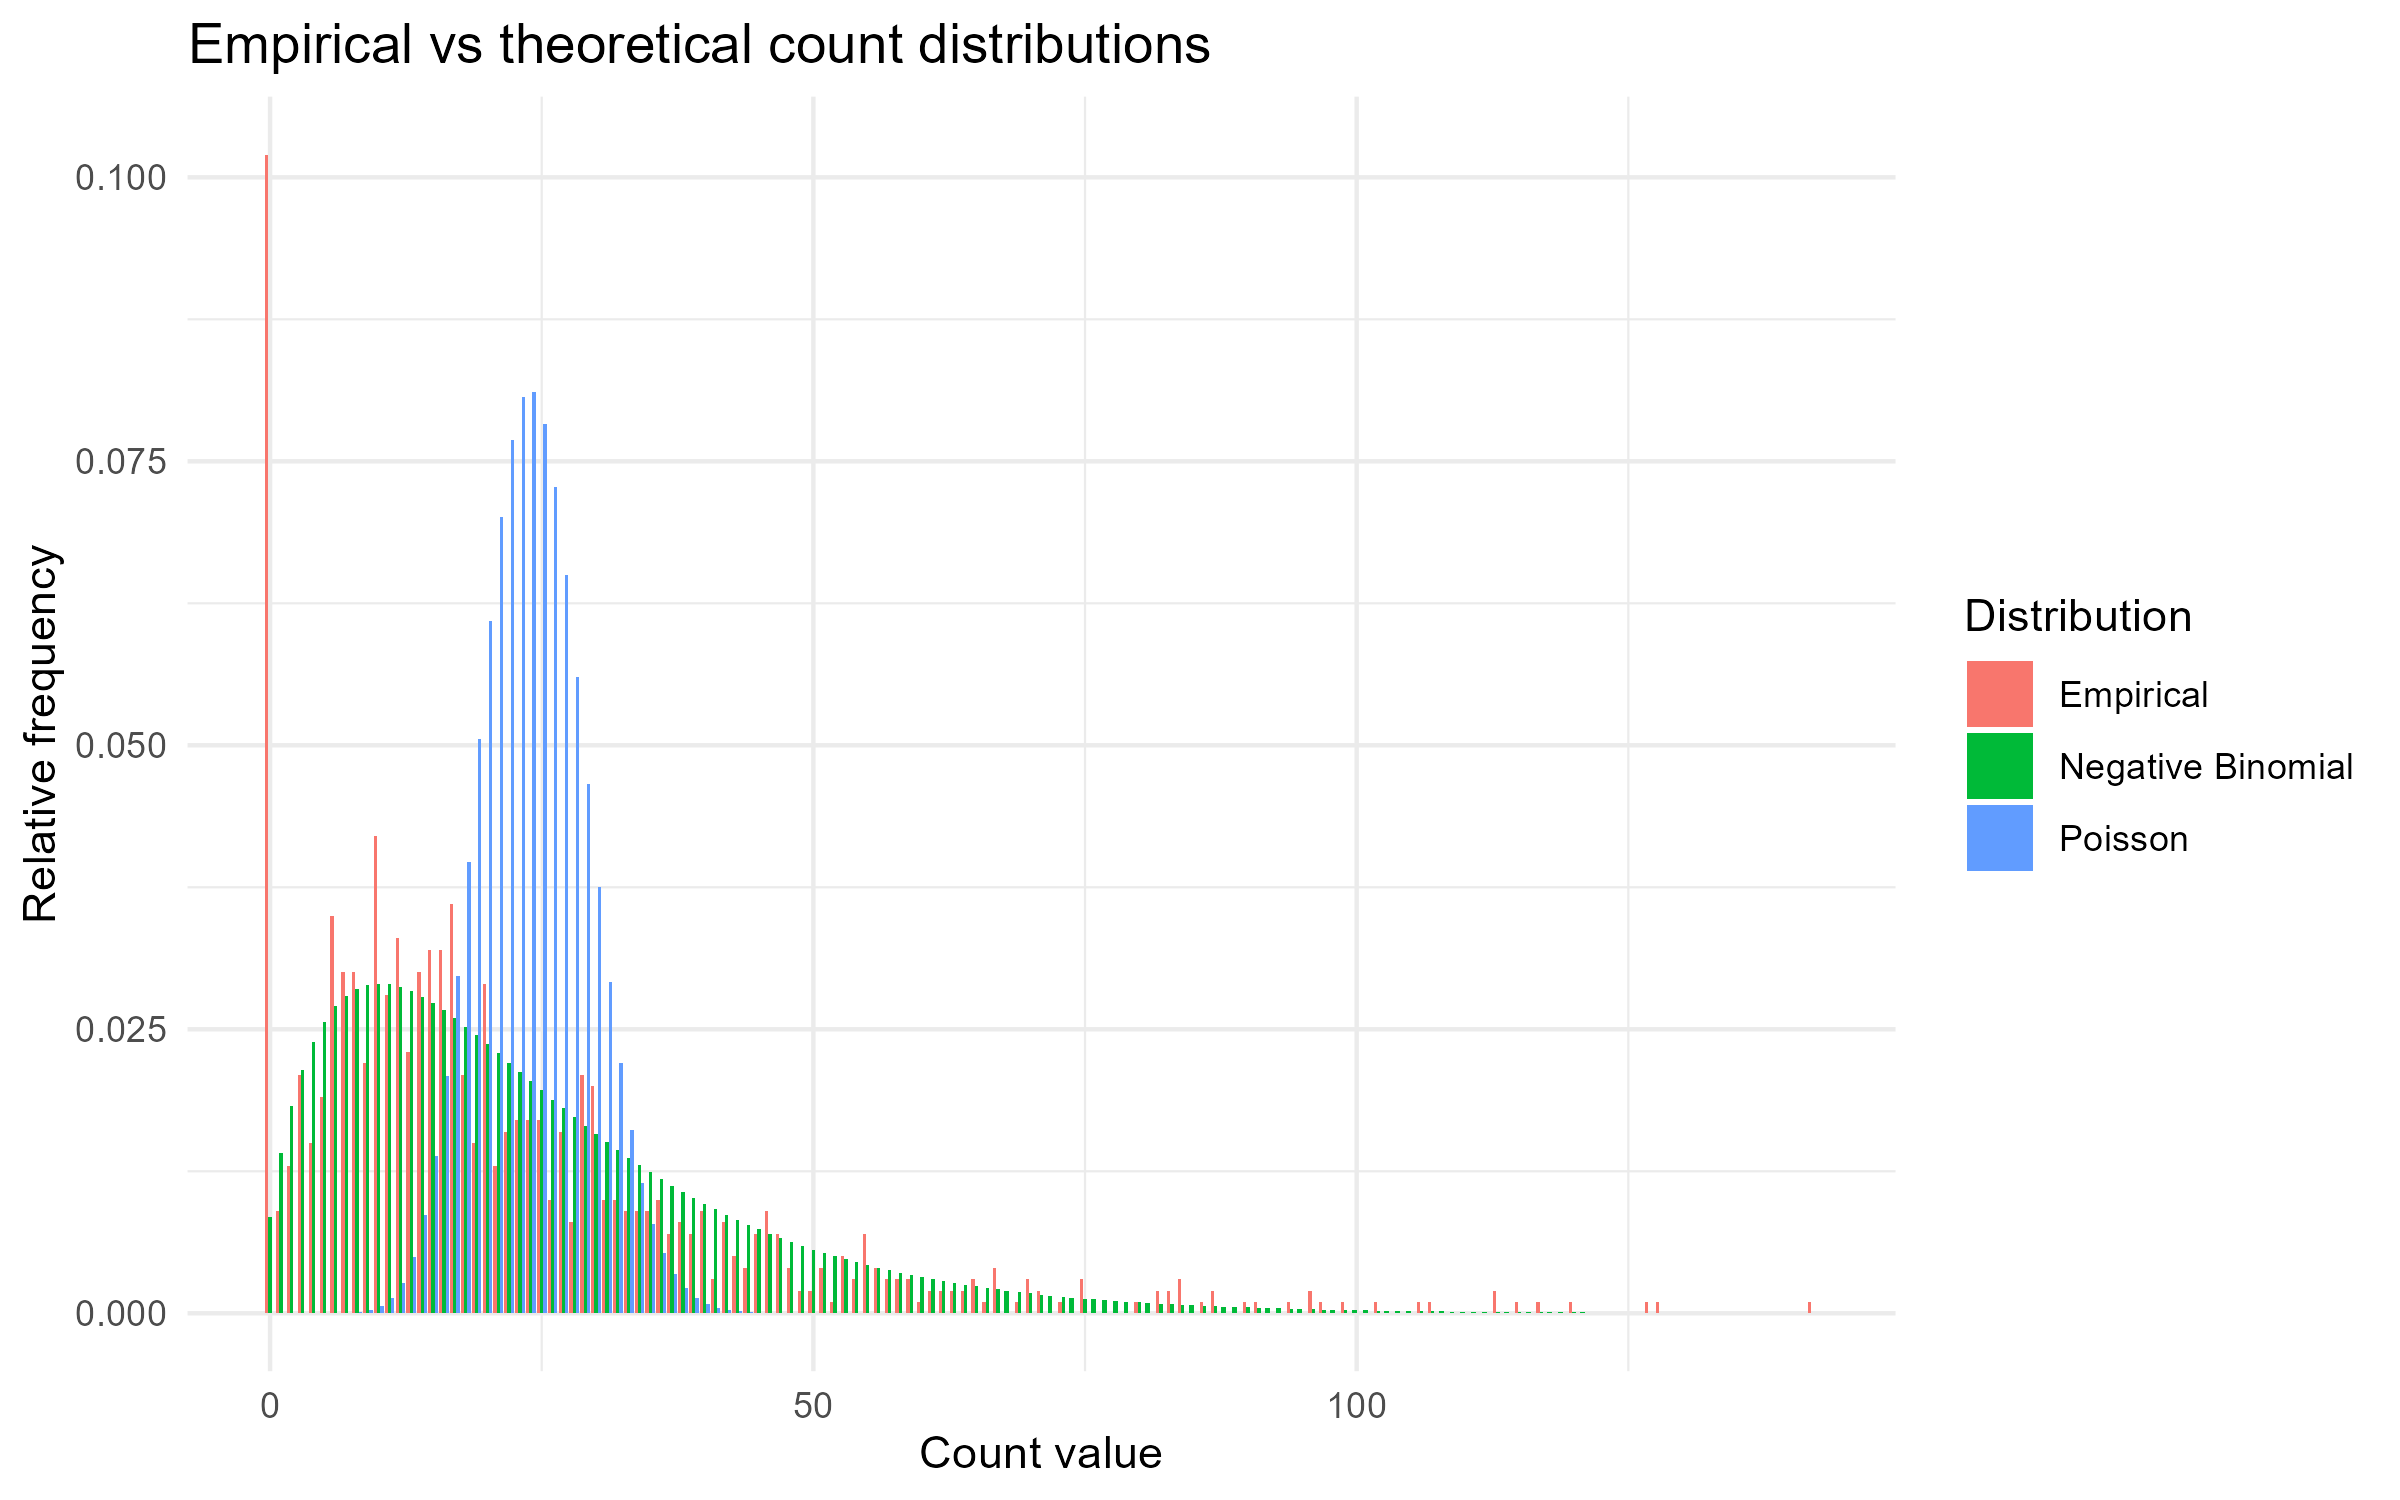
\includegraphics[width=0.9\textwidth]{figures/eda_count_distribution.png}
  \caption{Empirical relative frequencies compared with theoretical Poisson and
  negative binomial distributions.}
  \label{fig:eda}
\end{figure}

\section{Model fitting}

ZA and ZI models are fitted starting from saturated specifications and removing
variables with high individual $p$-values (non-significant coefficients). After
searching over count and zero-process distributions, the shortlisted ZA models
are:
\[
\texttt{zanbp\_x12f3\_x1235f2},\quad
\texttt{zanbb\_x12f3\_x5},\quad
\texttt{zapp\_x123f3\_x1235f2},\quad
\texttt{zapb\_x123f3\_x5}.
\]

Naming convention: \texttt{ZA} denotes a Zero-Altered (hurdle) model; the next
letter(s) give the count distribution (\texttt{nb} = negative binomial,
\texttt{p} = Poisson); the following letter is the zero-process distribution;
after the first underscore come the count-model covariates, and after the second
underscore the zero-model covariates. Thus
\texttt{zanbp\_x12f3\_x1235f2} is a ZA model with negative binomial counts,
Poisson zeros, covariates \texttt{x1}, \texttt{x2}, \texttt{factor3} in the
count part, and \texttt{x1}, \texttt{x2}, \texttt{x3}, \texttt{x5},
\texttt{factor2} in the zero part.

The shortlisted ZI models are:
\[
\texttt{zinb\_x12f3\_0f1},\quad
\texttt{zip\_x132f3\_0f1},\quad
\texttt{zinb\_x12f3\_1}.
\]
For ZI models only the count distribution is varied, given their theoretical
construction.

Goodness-of-fit comparisons show a substantial gap between ZA and ZI models
(Table~\ref{tab:model_comparison}): ZA models have markedly lower AIC/BIC and
recover a large share of the observed zeros, whereas the ZI candidates predict
none. This supports interpreting the sample zeros as arising from a single
process (structural / ``real'' zeros) rather than a separate inflation process.

\begin{table}[htbp]
  \centering
  \caption{Performance of shortlisted ZA and ZI models on the full sample,
  ordered by ascending AIC. Residual SD is the standard deviation of model
  residuals; predicted zeros count fitted values rounded to zero.}
  \label{tab:model_comparison}
  \small
  \begin{tabular}{lrrrrr}
\toprule
Model & Residual SD & AIC & BIC & Obs.\ zeros & Pred.\ zeros \\
\midrule
\texttt{zanbb\_x12f3\_x5} & 5.78 & 5432.7 & 5467.1 & 102 & 66 \\
\texttt{zanbp\_x12f3\_x1235f2} & 6.02 & 5453.1 & 5507.1 & 102 & 46 \\
\texttt{zapb\_x123f3\_x5} & 5.56 & 5453.5 & 5487.8 & 102 & 66 \\
\texttt{zapp\_x123f3\_x1235f2} & 5.80 & 5473.9 & 5527.9 & 102 & 46 \\
\texttt{zinb\_x12f3\_1} & 10.48 & 6035.0 & 6064.4 & 102 & 0 \\
\texttt{zinb\_x12f3\_0f1} & 10.48 & 6038.8 & 6078.1 & 102 & 0 \\
\texttt{zip\_x132f3\_0f1} & 10.42 & 6059.5 & 6098.7 & 102 & 0 \\
\bottomrule
\end{tabular}

\end{table}

\section{Model selection}

AIC and BIC are used for selection (avoiding reliance on the Vuong test). By
that criterion (Table~\ref{tab:model_comparison}) the best model is
\texttt{zanbb\_x12f3\_x5}, with the lowest AIC and BIC among the candidates.
It predicts 66 of the 102 zeros present in the sample. Figure~\ref{fig:diagnostics}
shows its diagnostic plots.

Predictions lie close to the observed counts, with more dispersion at larger
count values: low counts are predicted more accurately than high ones. Points
concentrate around the perfect-prediction line $y=x$. The residual standard
deviation is approximately $5.78$, which is relatively low given the range of
the response. Overall, the model is a good fit for this data set.

The exploratory analysis already suggested that the negative binomial would
match the empirical distribution best; the selected model indeed uses a
negative binomial count component.

\begin{figure}[htbp]
  \centering
  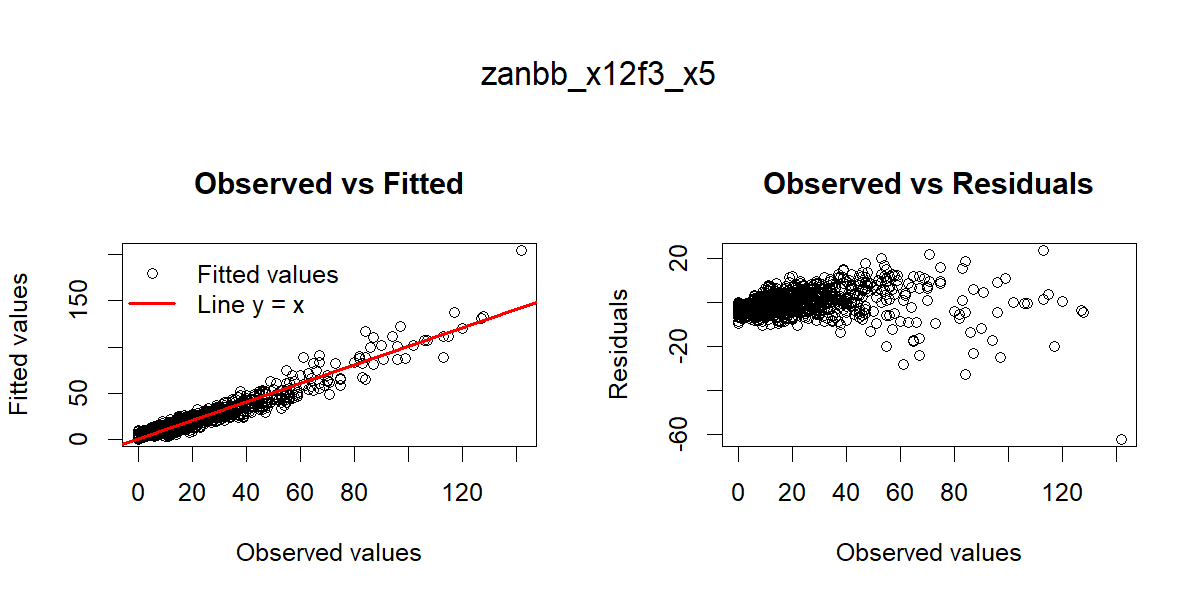
\includegraphics[width=0.95\textwidth]{figures/diagnostics_zanbb_x12f3_x5.png}
  \caption{Observed vs fitted and observed vs residuals for the selected model
  \texttt{zanbb\_x12f3\_x5}.}
  \label{fig:diagnostics}
\end{figure}

\section{Appendix: Code}

The full analysis script is
\texttt{notebooks/01\_count\_regression.R}. Running it from the project
directory loads
\texttt{data/raw/AEM\_02\_Count\_regression\_and\_GAM.xlsx}, fits the ZA/ZI
models, writes the comparison table under \texttt{tables/}, and regenerates
the figures under \texttt{figures/} used in this report.

\end{document}
